\section{Validation}
\label{section:validation}
We start by validating our Schwarz-SEM framework against a commonly-used nonspinning circle monodomain SEM case. We ran monodomain and Schwarz-SEM simulations in domains of size 43x24. In these validation cases, our parameter space is $\{\Rey, \Pran, AR, \Omega^{\ast}\} = \{120, 1, 1, 0\}$. Figure \ref{fig:nn val} compares the drag coefficient, which is calculated as $C_D = 2F_D$. We only see a slight disagreement at $Fr^2 = 0.01$, which comes out to an error of less than $3.1\%$.  

\begin{figure}
    \centerline{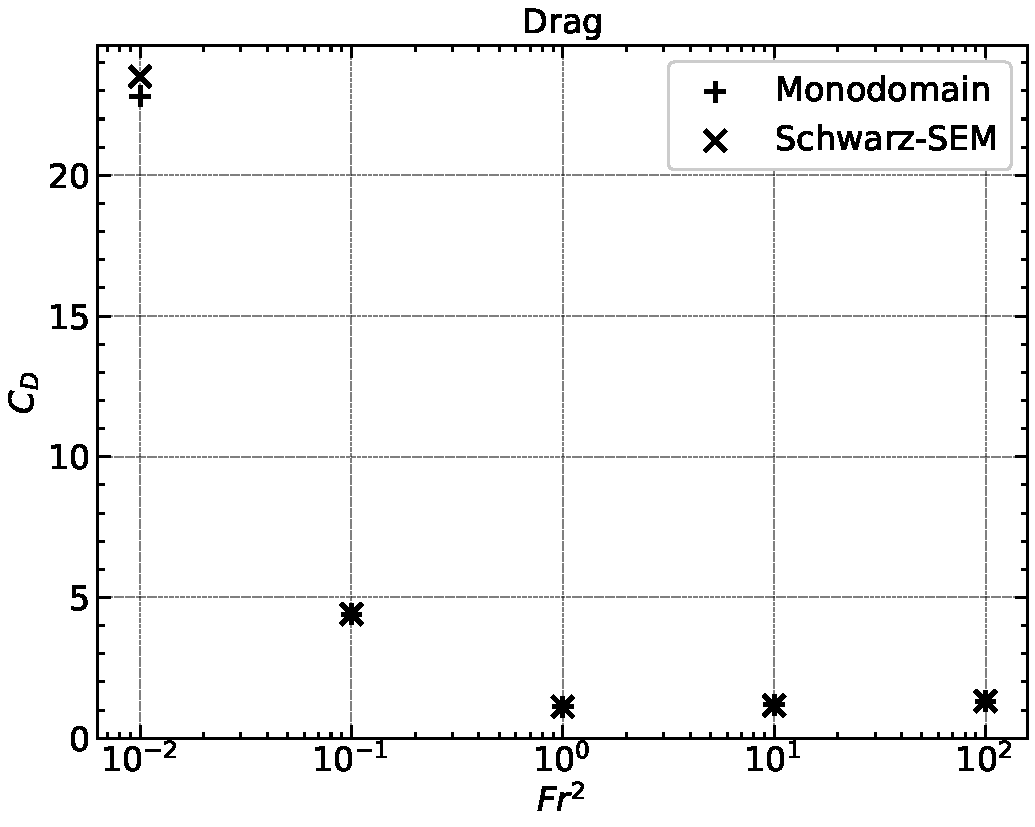
\includegraphics[width=.8\textwidth]{images/dragvalnn.pdf}}
    \caption{Validation of the Schwarz-SEM framework at $\Omega^{\ast}$ for stratified flow}
    \label{fig:nn val}
\end{figure}

Now that the nonspinning stratified Schwarz-SEM for circular shapes has been validated, we move to validating the nonstratified, elliptical Schwarz-SEM framework. We compare our drag and lift results with those of two papers, Lu et al. \cite{lu_flow_2018} and Lua et al. \cite{lua_rotating_2018}. Our domain dimensions and boundary conditions matched. Figure \ref{fig:lua_com} shows the drag and lift results between us and the two papers. Interestingly, the net thrust observed by the two papers is also observed in our results.
\begin{figure}
    \centering
    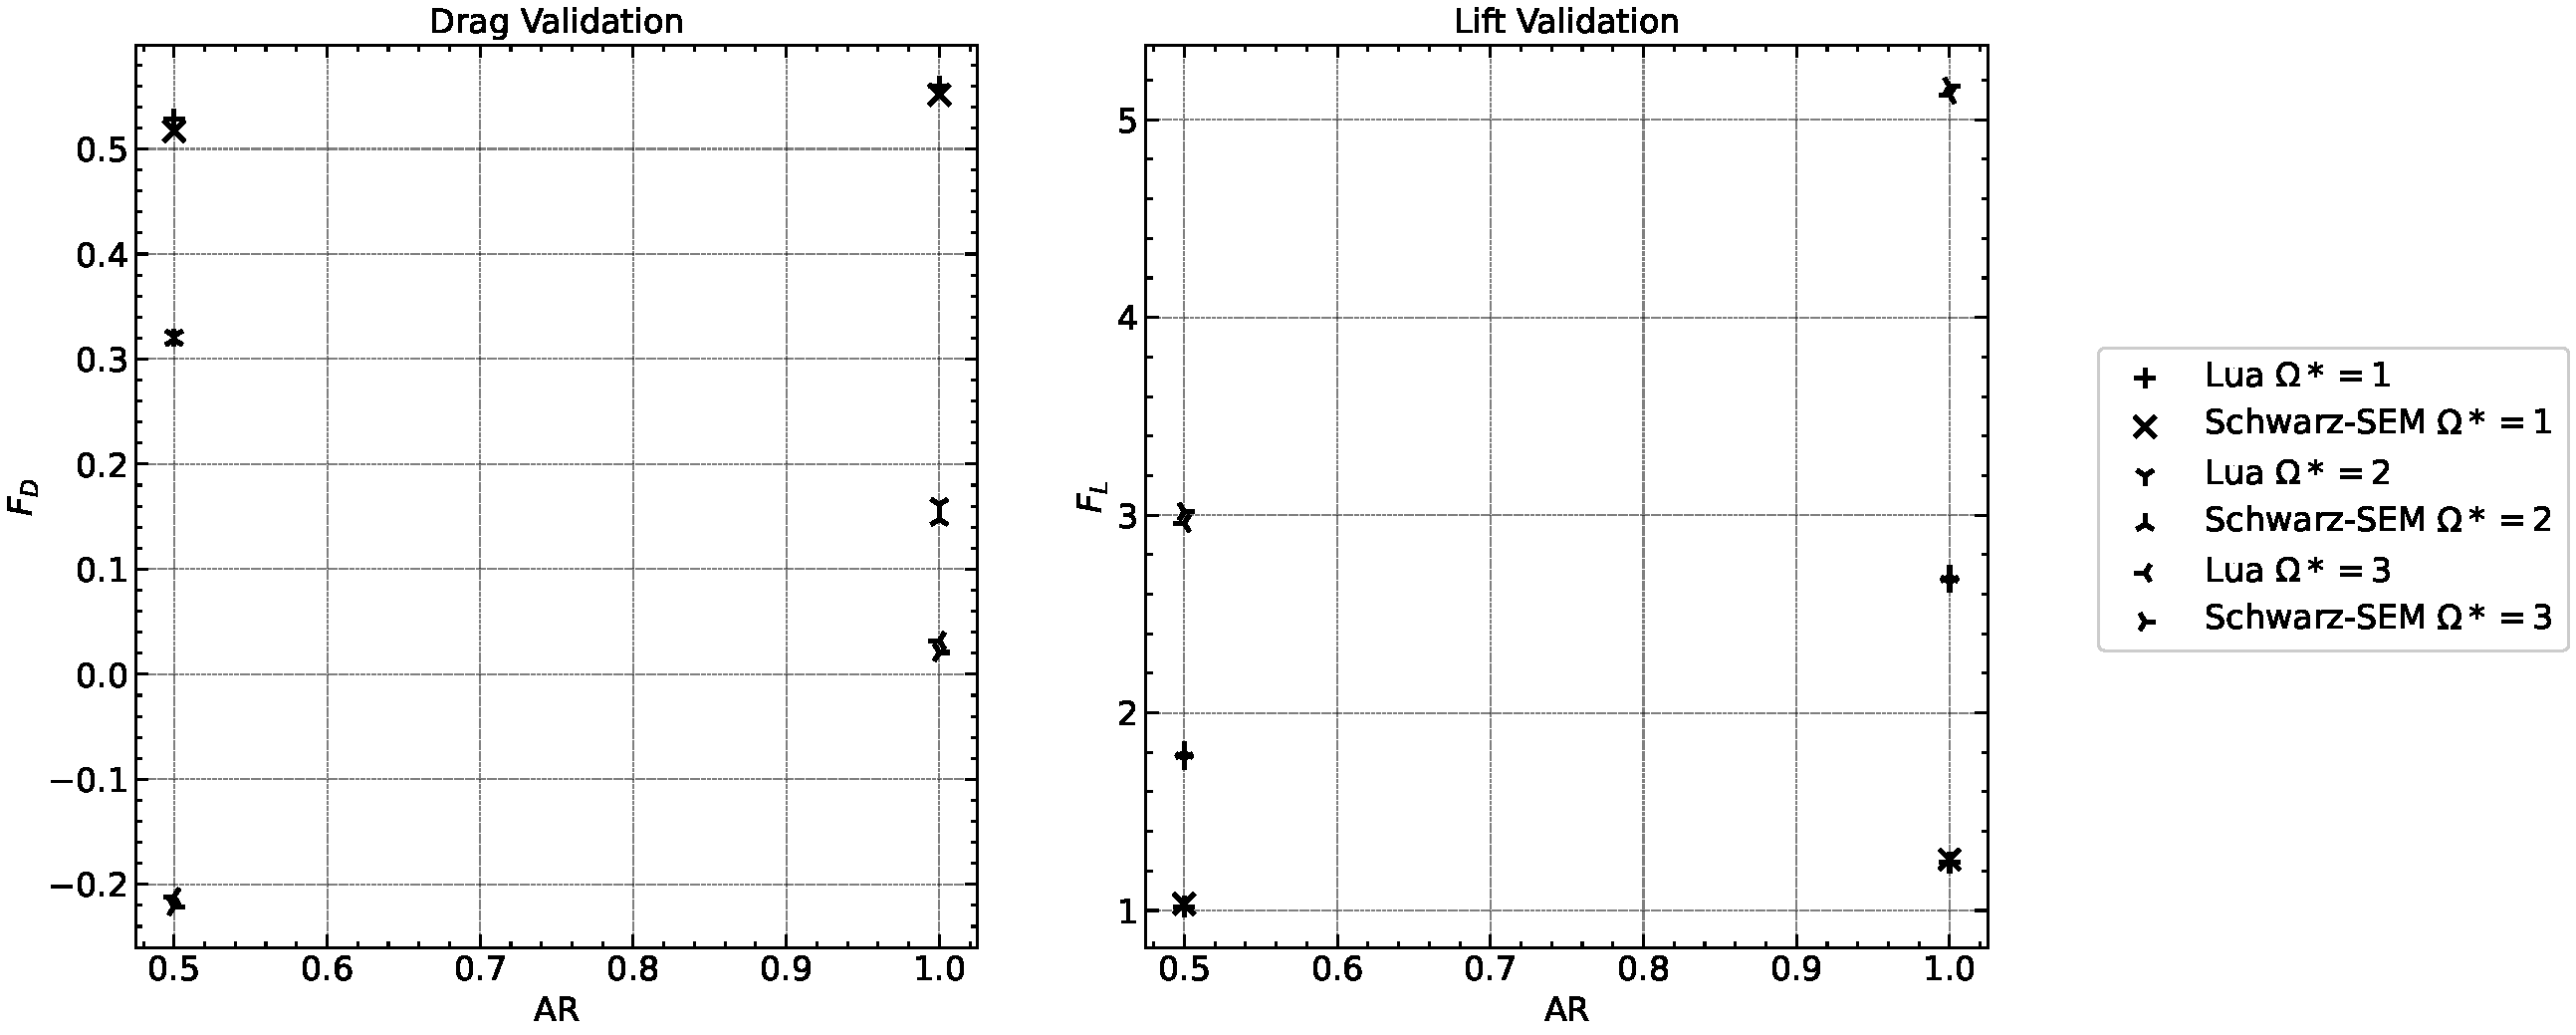
\includegraphics[width=\textwidth]{lua_com.pdf}
    \caption{Comparison against Lu et al. \cite{lu_flow_2018} and Lua et al. \cite{lua_rotating_2018}}
    \label{fig:lua_com}
\end{figure}
While conducting these validation tests, it was found that at higher rotation rates, the drag values are more sensitive to domain size and lateral boundary conditions. This is a topic that is not discussed much in the literature; domain size and lateral boundary conditions are not given much consideration. 

Figure \ref{fig:domain_conv} shows that in the case of $\Omega^{\ast} = 3$, there is a large discrepancy in drag at height $H = 40D$ between the two boundary condition types. We also see that as we change the domain size, regardless of boundary condition, the drag also changes.  However, there is a vertical length of convergence for domain size. For the case of $\Omega^{\ast} = 3$, we observe a convergence towards a value of about $120D$. Interestingly, the variance is higher in the case of the periodic boundary conditions than the symmetric boundary conditions. The figure also shows that there is also a vertical length of convergence where the drag for the periodic and symmetric boundary condition cases converge. The required height increases with rotational velocity, as expected. 
\begin{figure}
    \centerline{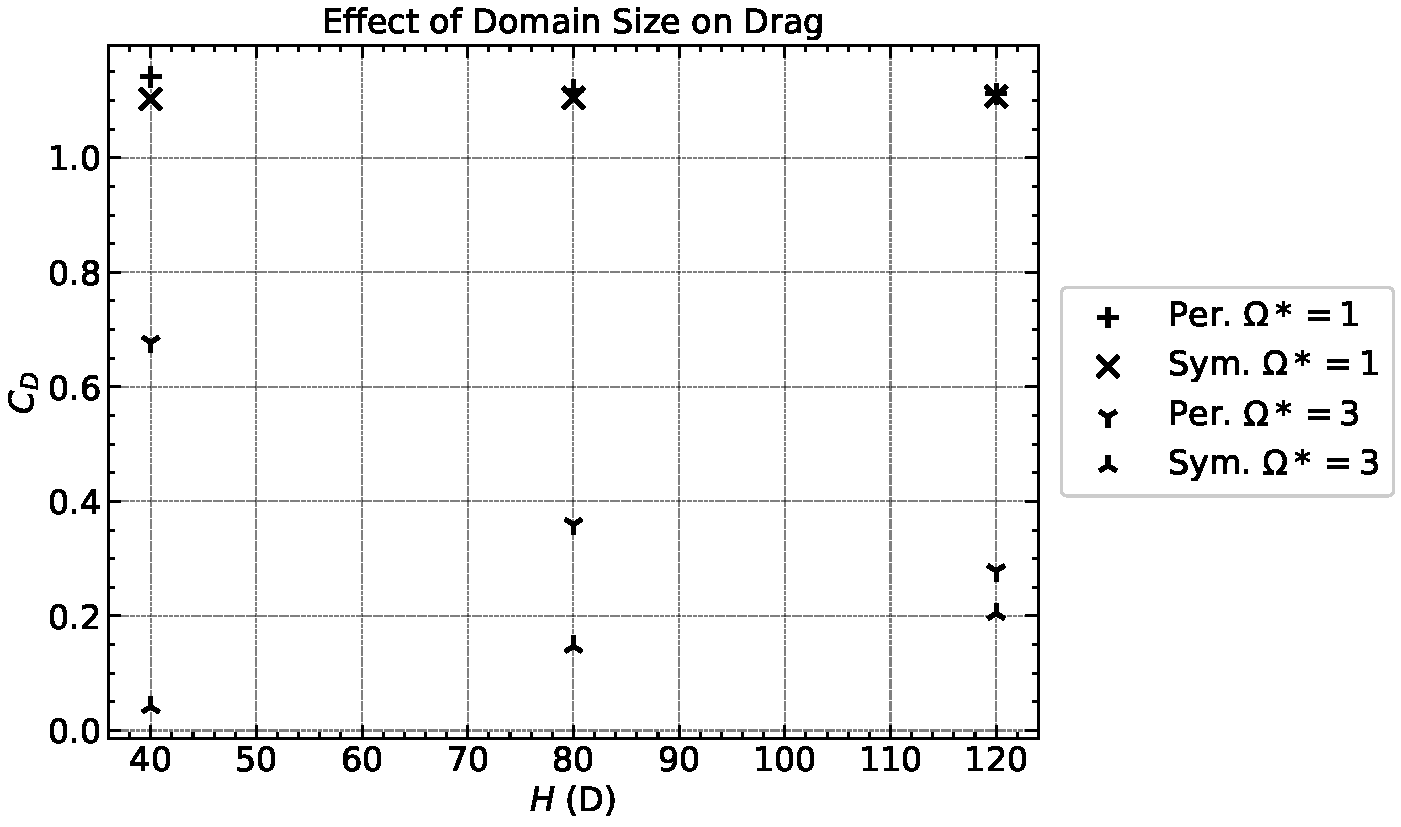
\includegraphics[width=.9\textwidth]{domain_conv.pdf}}
    \caption{At higher rotation speeds, larger domain sizes are required}
    \label{fig:domain_conv}
\end{figure}
In Fig. \ref{fig:per}, we see how in the case of the periodic boundary conditions, the rotation of the cylinder is able to redirect the flow down since the periodic boundary conditions allow for flow normal to the boundaries; the flow comes done from the top, further redirecting the flow. This does not happen in the case of the symmetric boundary conditions, as Fig. \ref{fig:sym} shows. Because there is no flow normal to the boundaries at the boundaries, there is no flow rotation like there is in the case of the periodic boundary conditions. 
\begin{figure}
    \centering
    \begin{subfigure}{0.49\textwidth}
    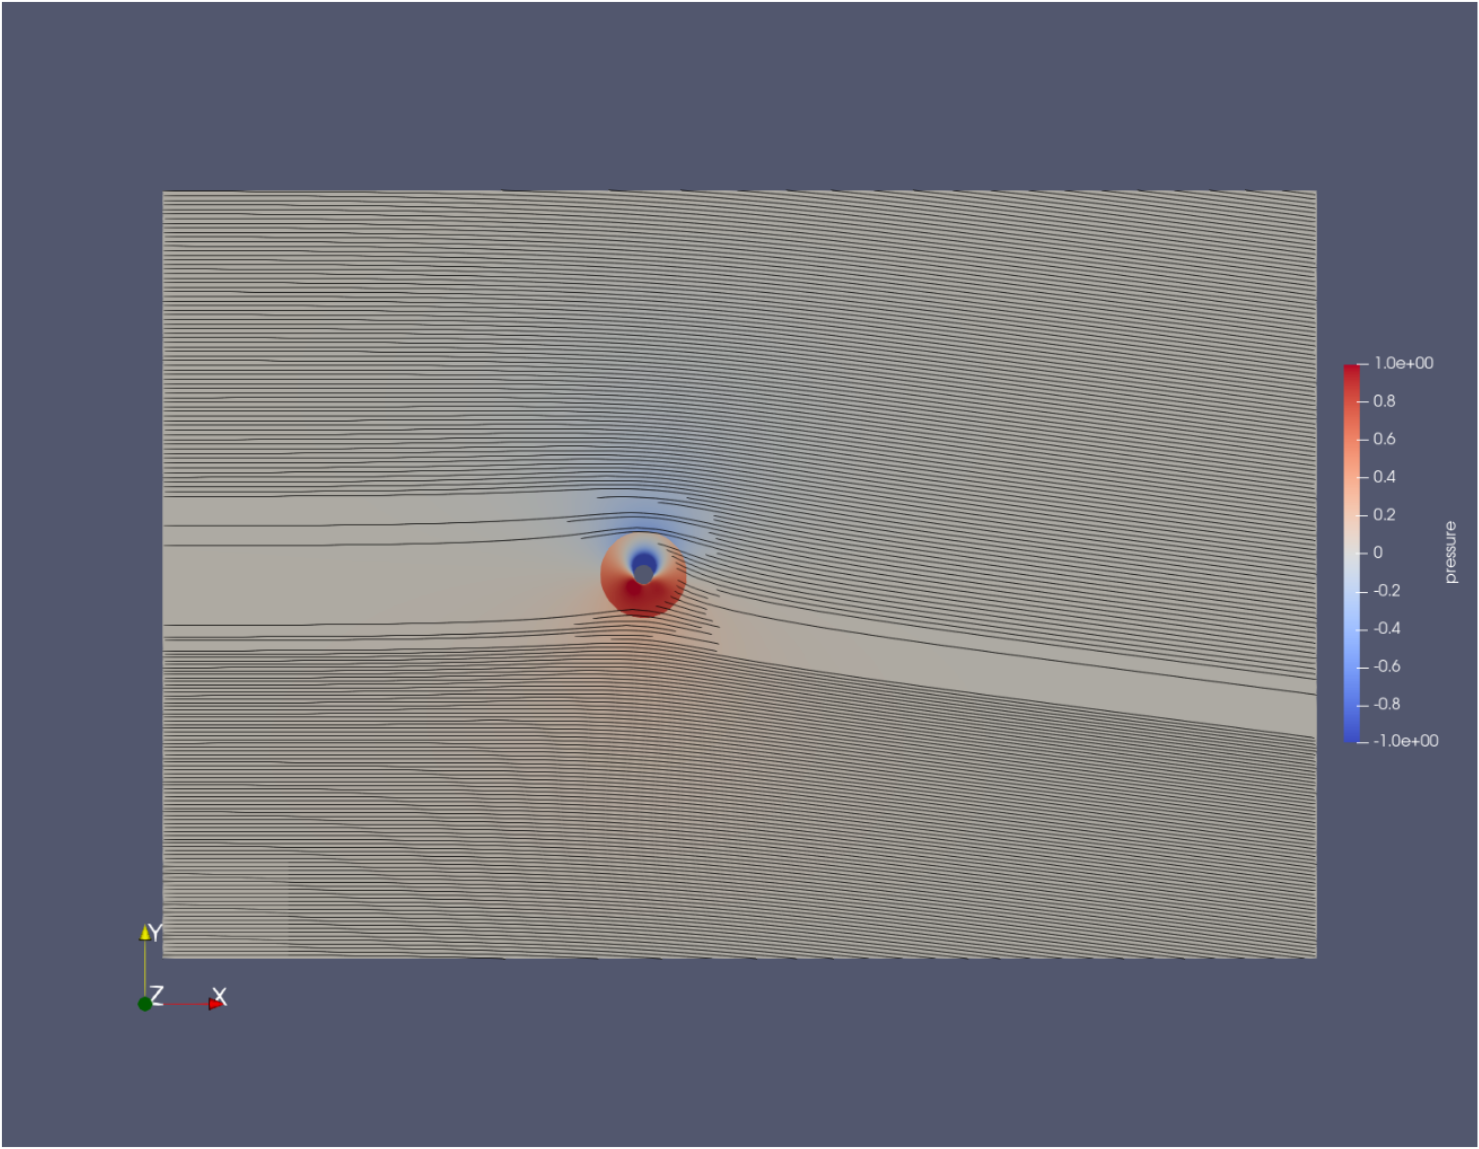
\includegraphics[width=\textwidth]{per.png}
    \caption{Periodic boundary conditions}
    \label{fig:per}
    \end{subfigure}
    \begin{subfigure}{0.49\textwidth}
    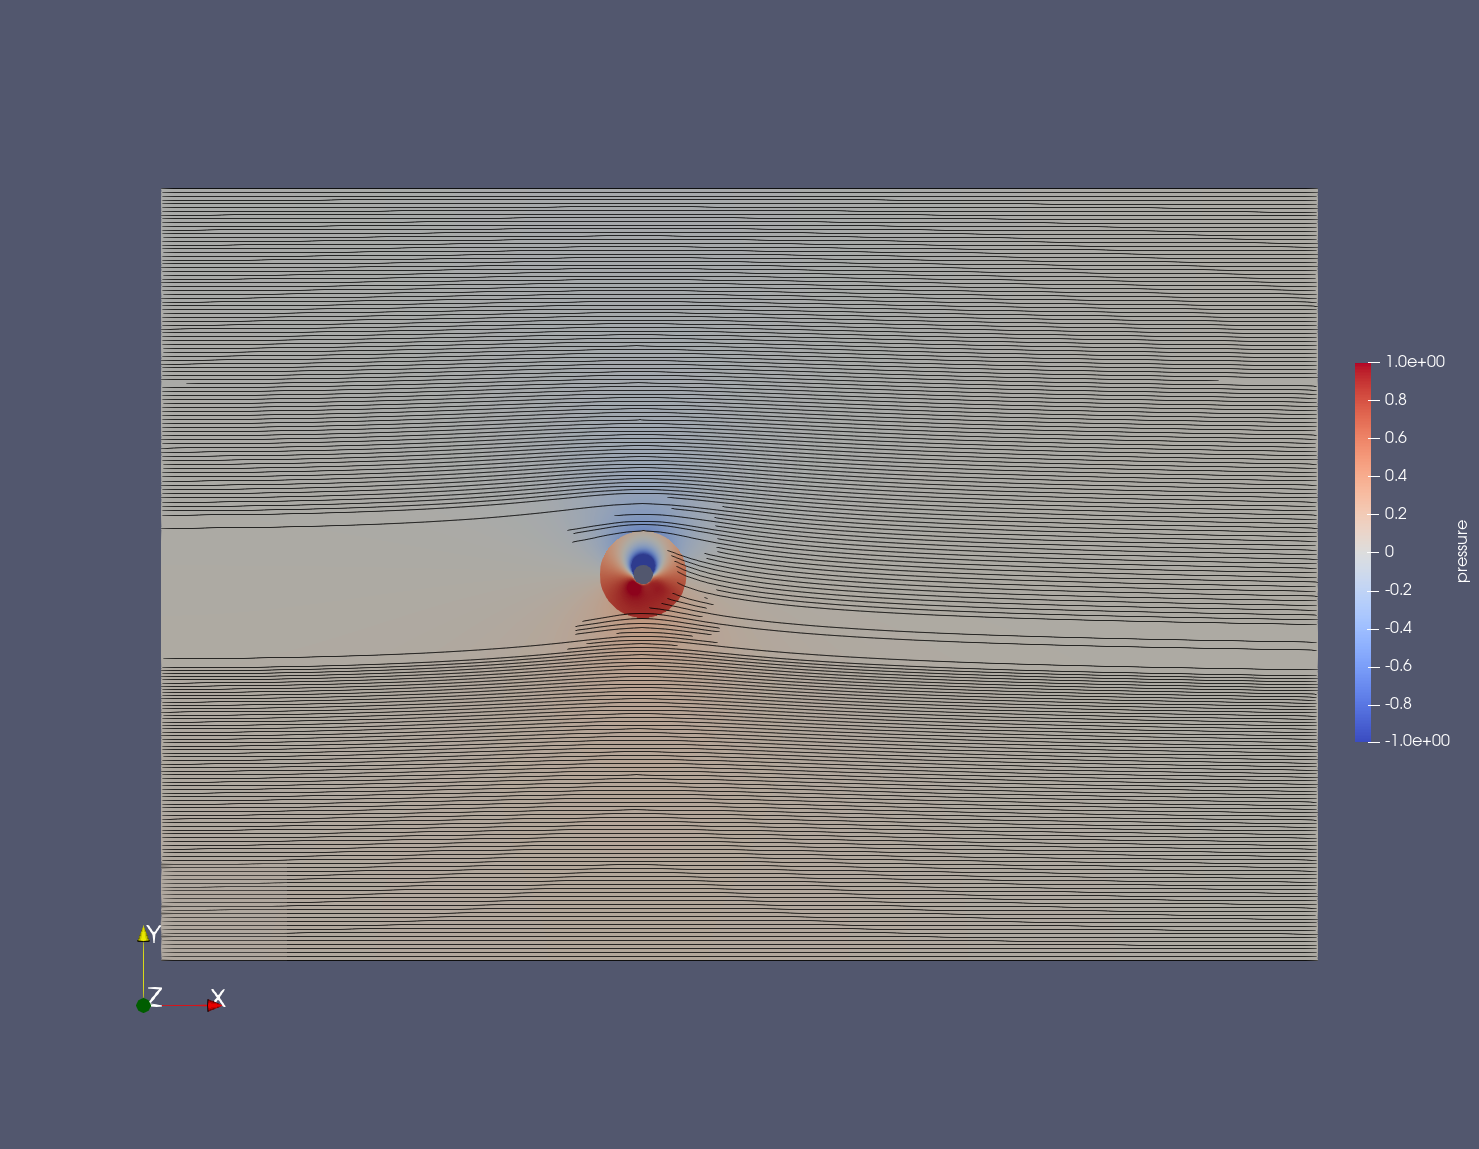
\includegraphics[width=\textwidth]{sym.png}
    \caption{Symmetric boundary conditions}
    \label{fig:sym}
    \end{subfigure}
    \caption{Pressure and streamline plots at $H = 40D$, $\Omega^{\ast} = 3$, $\Rey = 200$, aspect ratio = 1}
    \label{fig:per sym}
\end{figure}
The flow rotation in the case of the periodic boundary conditions also rotates the pressure distribution, as Fig. \ref{fig:polar pres} shows. The clockwise rotation of the negative pressure zone at the top creates a net increase in drag.
\begin{figure}
    \centerline{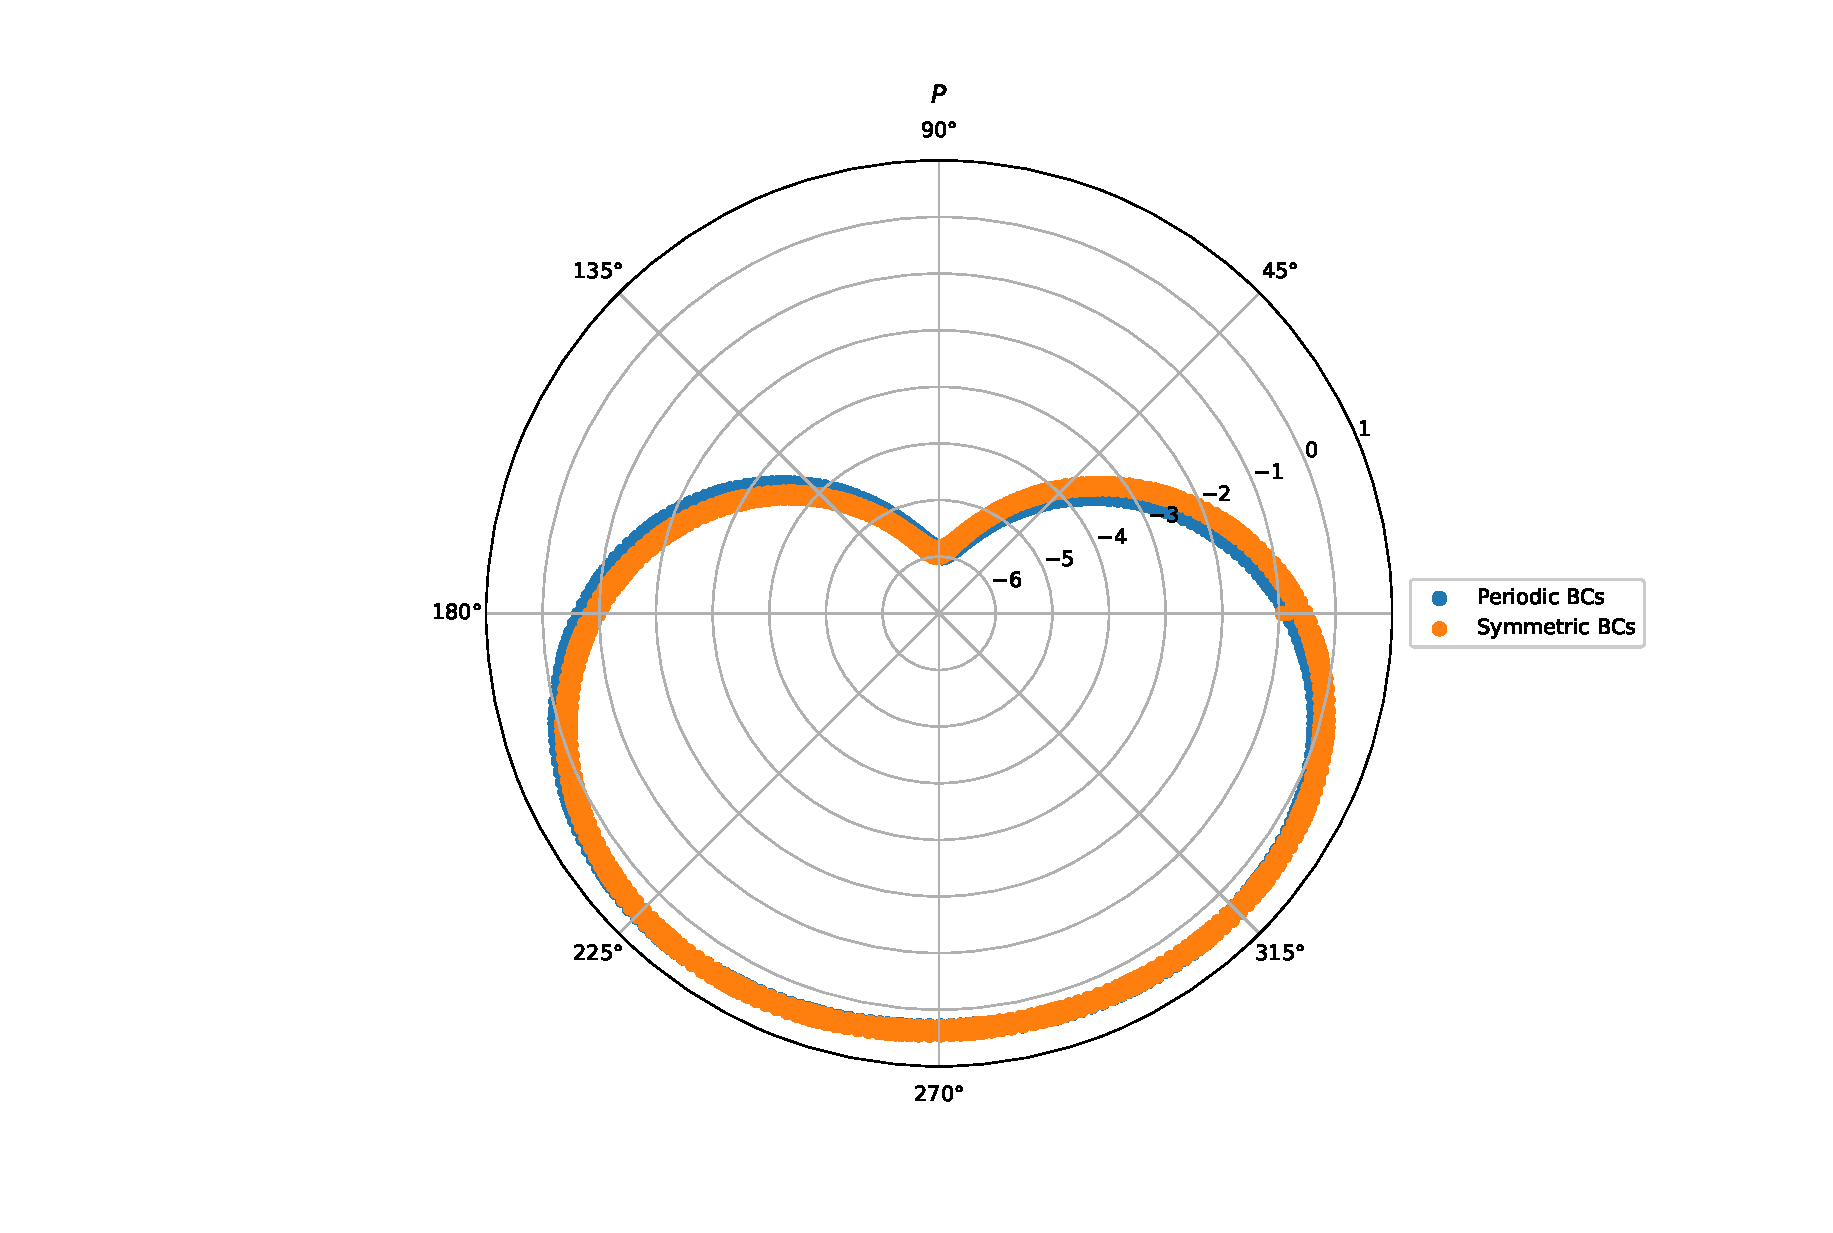
\includegraphics[width=0.9\textwidth]{polar.eps}}
    \caption{Polar plot of pressure on each surface at $\Omega^{\ast} = 3$}
    \label{fig:polar pres}
\end{figure}
The fact that the discrepancy in drag arises from the rotation of the low-pressure region explains why the drag discrepancy increases with higher rotational velocity. We now look at domains with larger heights to observe the effect of height on these discrepencies.

Figure \ref{fig:per12} shows that the rotation of the fluid is decreased as the domain height is increased. When you use periodic boundary conditions, you are in reality simulating an array (one-dimensional in this case) of cylinders. When you decrease domain heights, you increase the effect of "neighboring" cylinders on the flow. These virtual neighbors help induce more rotation in the flow. This is why there is a decrease in flow rotation with larger domain heights, which results in less negative-pressure region rotation. Less negative-pressure region rotation leads to an decrease in drag.  

In the symmetric boundary condition case, Fig. \ref{fig:sym12} shows how more rotation of the flow is allowed because the lateral boundaries are farther away from the body. This added rotation explains how the drag increases with domain size, as Fig. \ref{fig:domain_conv} shows.  
\begin{figure}
    \centering
    \begin{subfigure}{0.49\textwidth}
    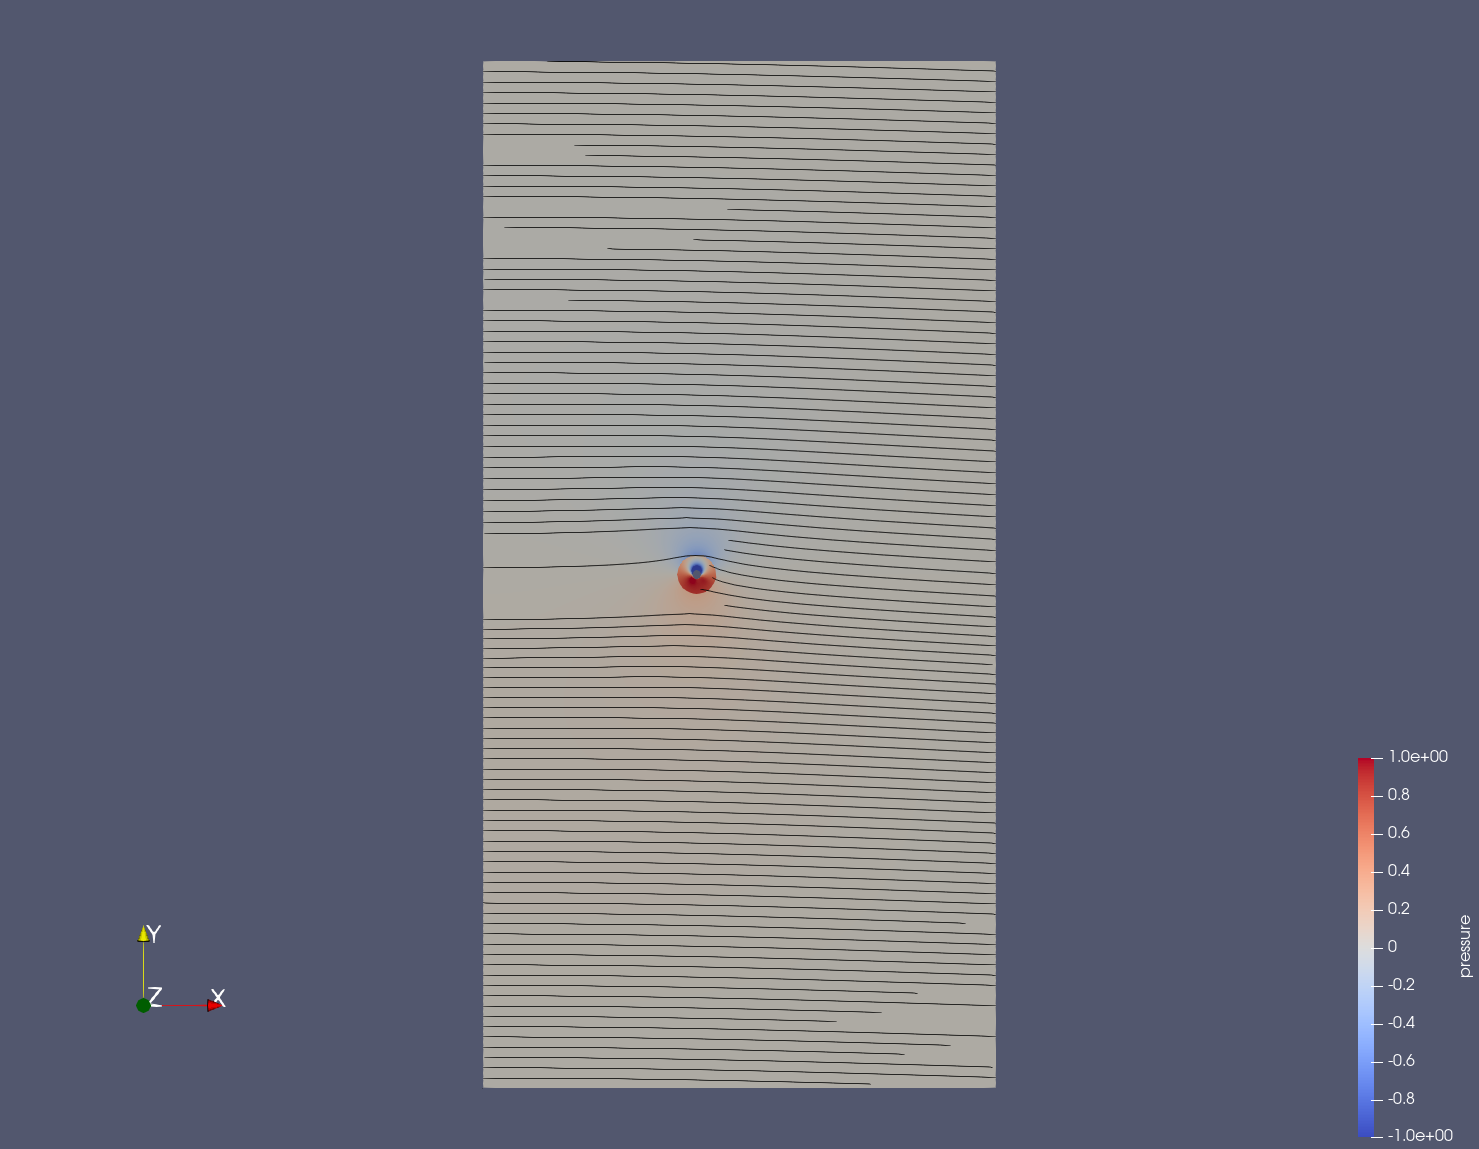
\includegraphics[width=\textwidth]{per12.png}
    \caption{Periodic boundary conditions}
    \label{fig:per12}
    \end{subfigure}
    \begin{subfigure}{0.49\textwidth}
    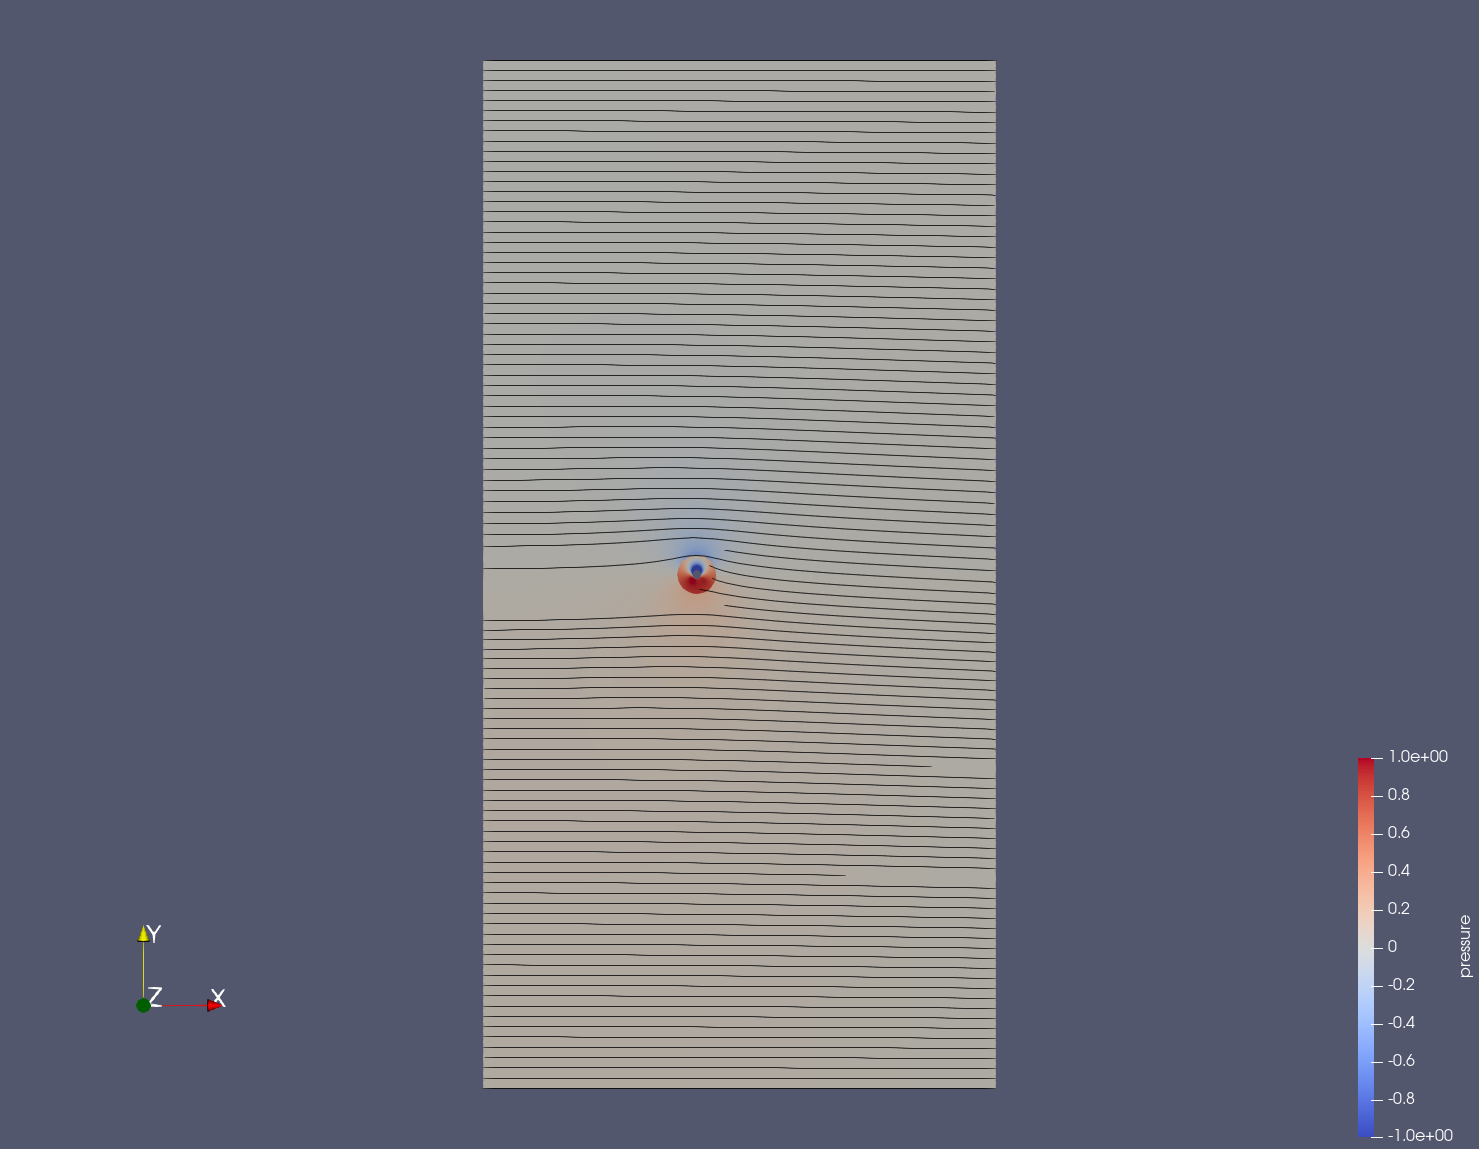
\includegraphics[width=\textwidth]{sym12.png}
    \caption{Symmetric boundary conditions}
    \label{fig:sym12}
    \end{subfigure}
    \caption{Pressure and streamline plots at $H=120D$, $\Omega^{\ast} = 3$, $\Rey = 200$, $AR = 1$}
    \label{fig:per sym12}
\end{figure}

Mittal and Kumar \cite{mittal_flow_2003} conducted a similar test looking only at symmetric boundary conditions. They conducted a study by varying the side length of a square mesh with a cylinder in the middle. They found that the drag values converge when the size of the domain is increased, which is consistent with our findings. However, their study changed both dimensions of the domain at the same time. Our study isolates the effect of the height of the domain. They did also find that lift is unaffected by domain size, which is consistent with our results. 

We perform a similar analysis with respect to a case at the edge of our parameter space where $Fr^2 = 0.01$, $AR = 1.5$, $\Omega^{\ast}$ as Fig. \ref{fig:high_strat_mesh} shows. 
\begin{figure}
	\centerline{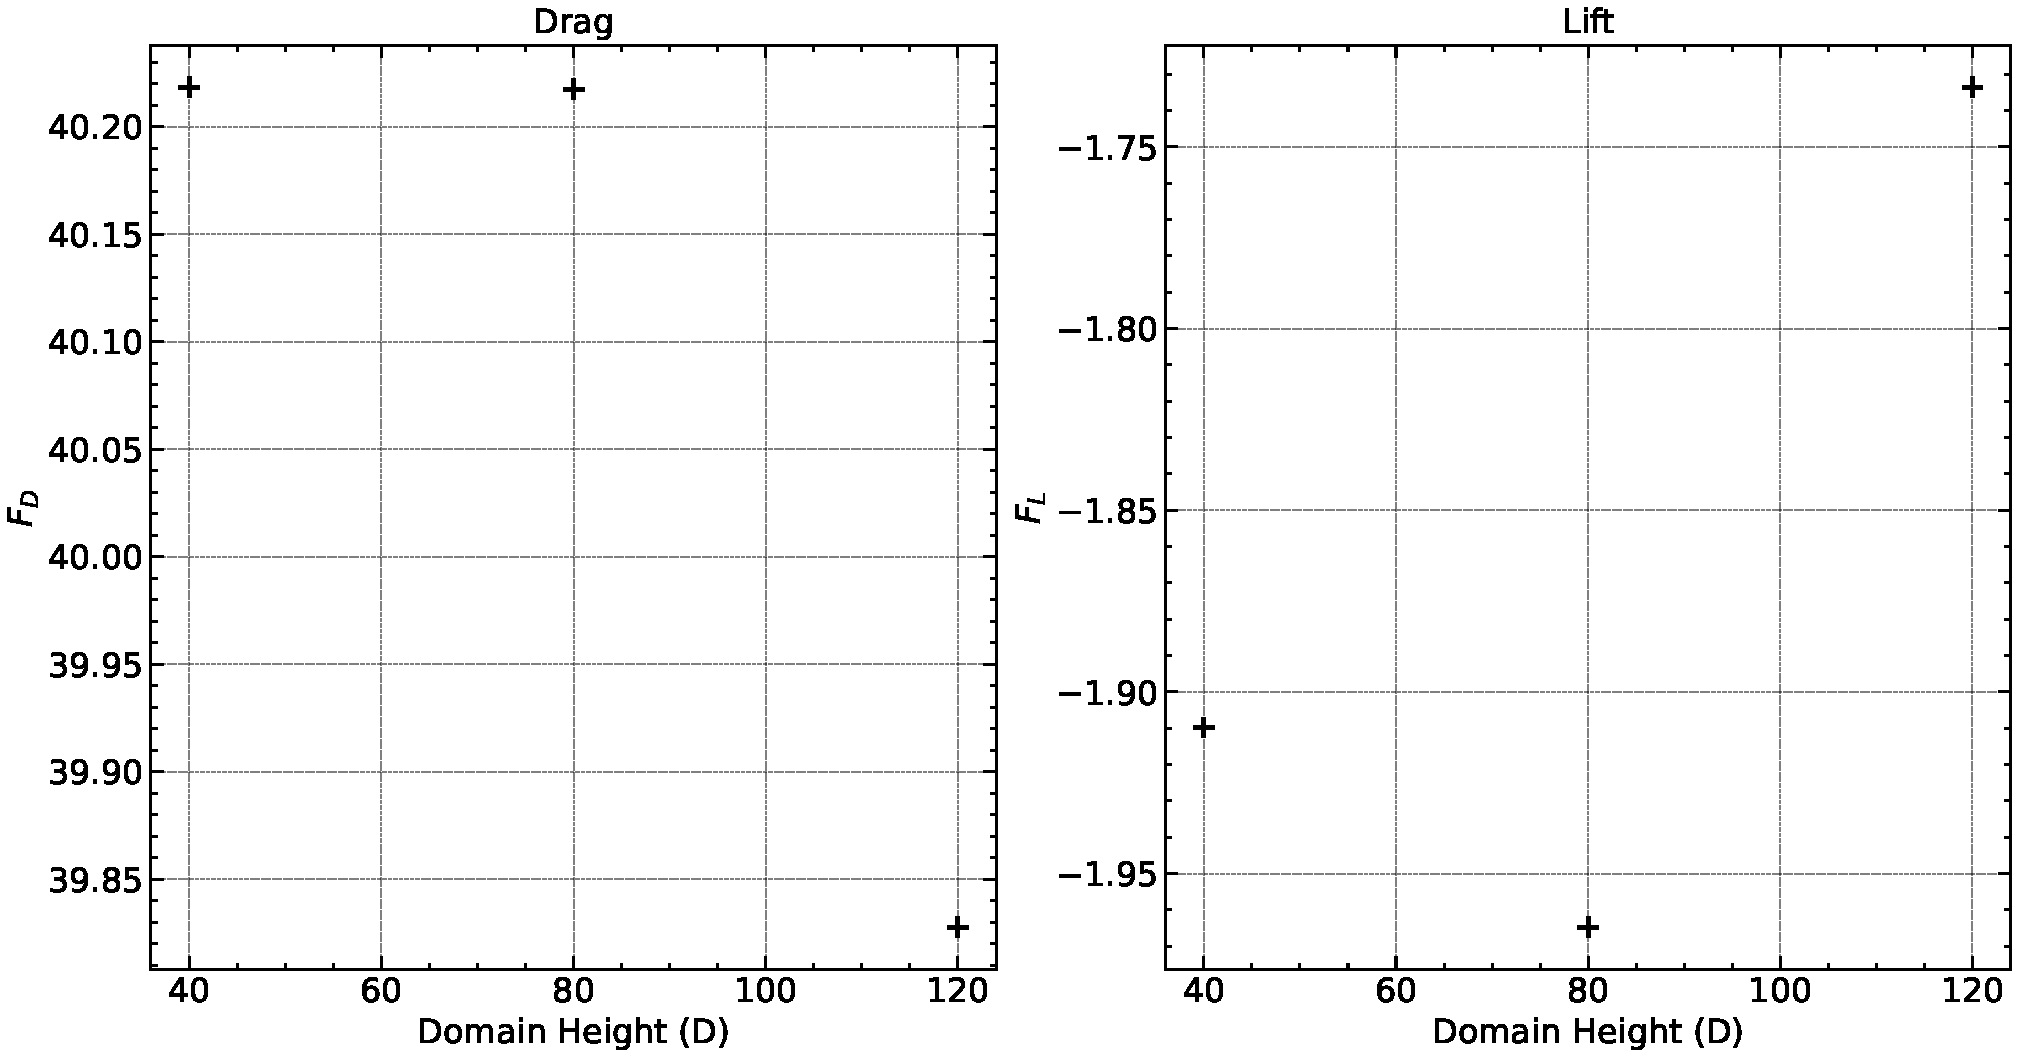
\includegraphics[width=\textwidth]{images/spinning_ellipse/high_strat_mesh.pdf}}
	\caption{Effect of domain size at $Fr^2 = 0.01$, $AR = 1.5$, $\Omega^{\ast}$}
	\label{fig:high_strat_mesh}
\end{figure}
An interesting pattern is how the two shorter domains produce closer drag and lift values than the $H = 120D$ case. Figure \ref{fig:strat_mesh} shows how the extended vertical boundaries allow the IGW to travel more freely.   
\begin{figure}
	\centerline{\includegraphics[width=\textwidth]{images/spinning_ellipse/strat_mesh.png}}
	\caption{Vertical velocity plots of $H = 40D$ and $H = 120D$ cases}
	\label{fig:strat_mesh}
\end{figure}

We ran our simulations with polynomial order $N = 11$. We ran a case with $N = 9, 11, 13$ which, on a grid of $E = 3712$ elements, correspond to gridpoint counts between $n = E \cdot 9^2 = 300,672$ and $n = E \cdot 13^2 = 627,328$. The change in drag is less than $1\%$ and the change in lift is less than $2\%$. The mesh independence cases were conducted on the $Fr^2 = 0.01$, $AR = 1.5, \Omega^{\ast}$ case.

